\section{Results}
This section presents the results of Brazilian case study. With regard to evaluating the models, Figure \ref{fig:auc_ks2_max} presents the Area under ROC curve (AUC\_ROC)\cite{Fawcett2006AnAnalysis} and the maximum distance between Kolmogorov-Smirnov curves(  KS2\_max)\cite{kolmogorov1933sulla}. Both metrics achieved good results, with RF outperforming LR with a slight difference in both metrics over the whole period (1\% for AUC and 4\% for KS2\_Max in the period). 

\begin{figure}[ht!]
\centering
\caption{\textmd{AUC and KS2\_max of logistic regression and random forest models}}
\label{fig:auc_ks2_max}
\fcolorbox{gray}{white}{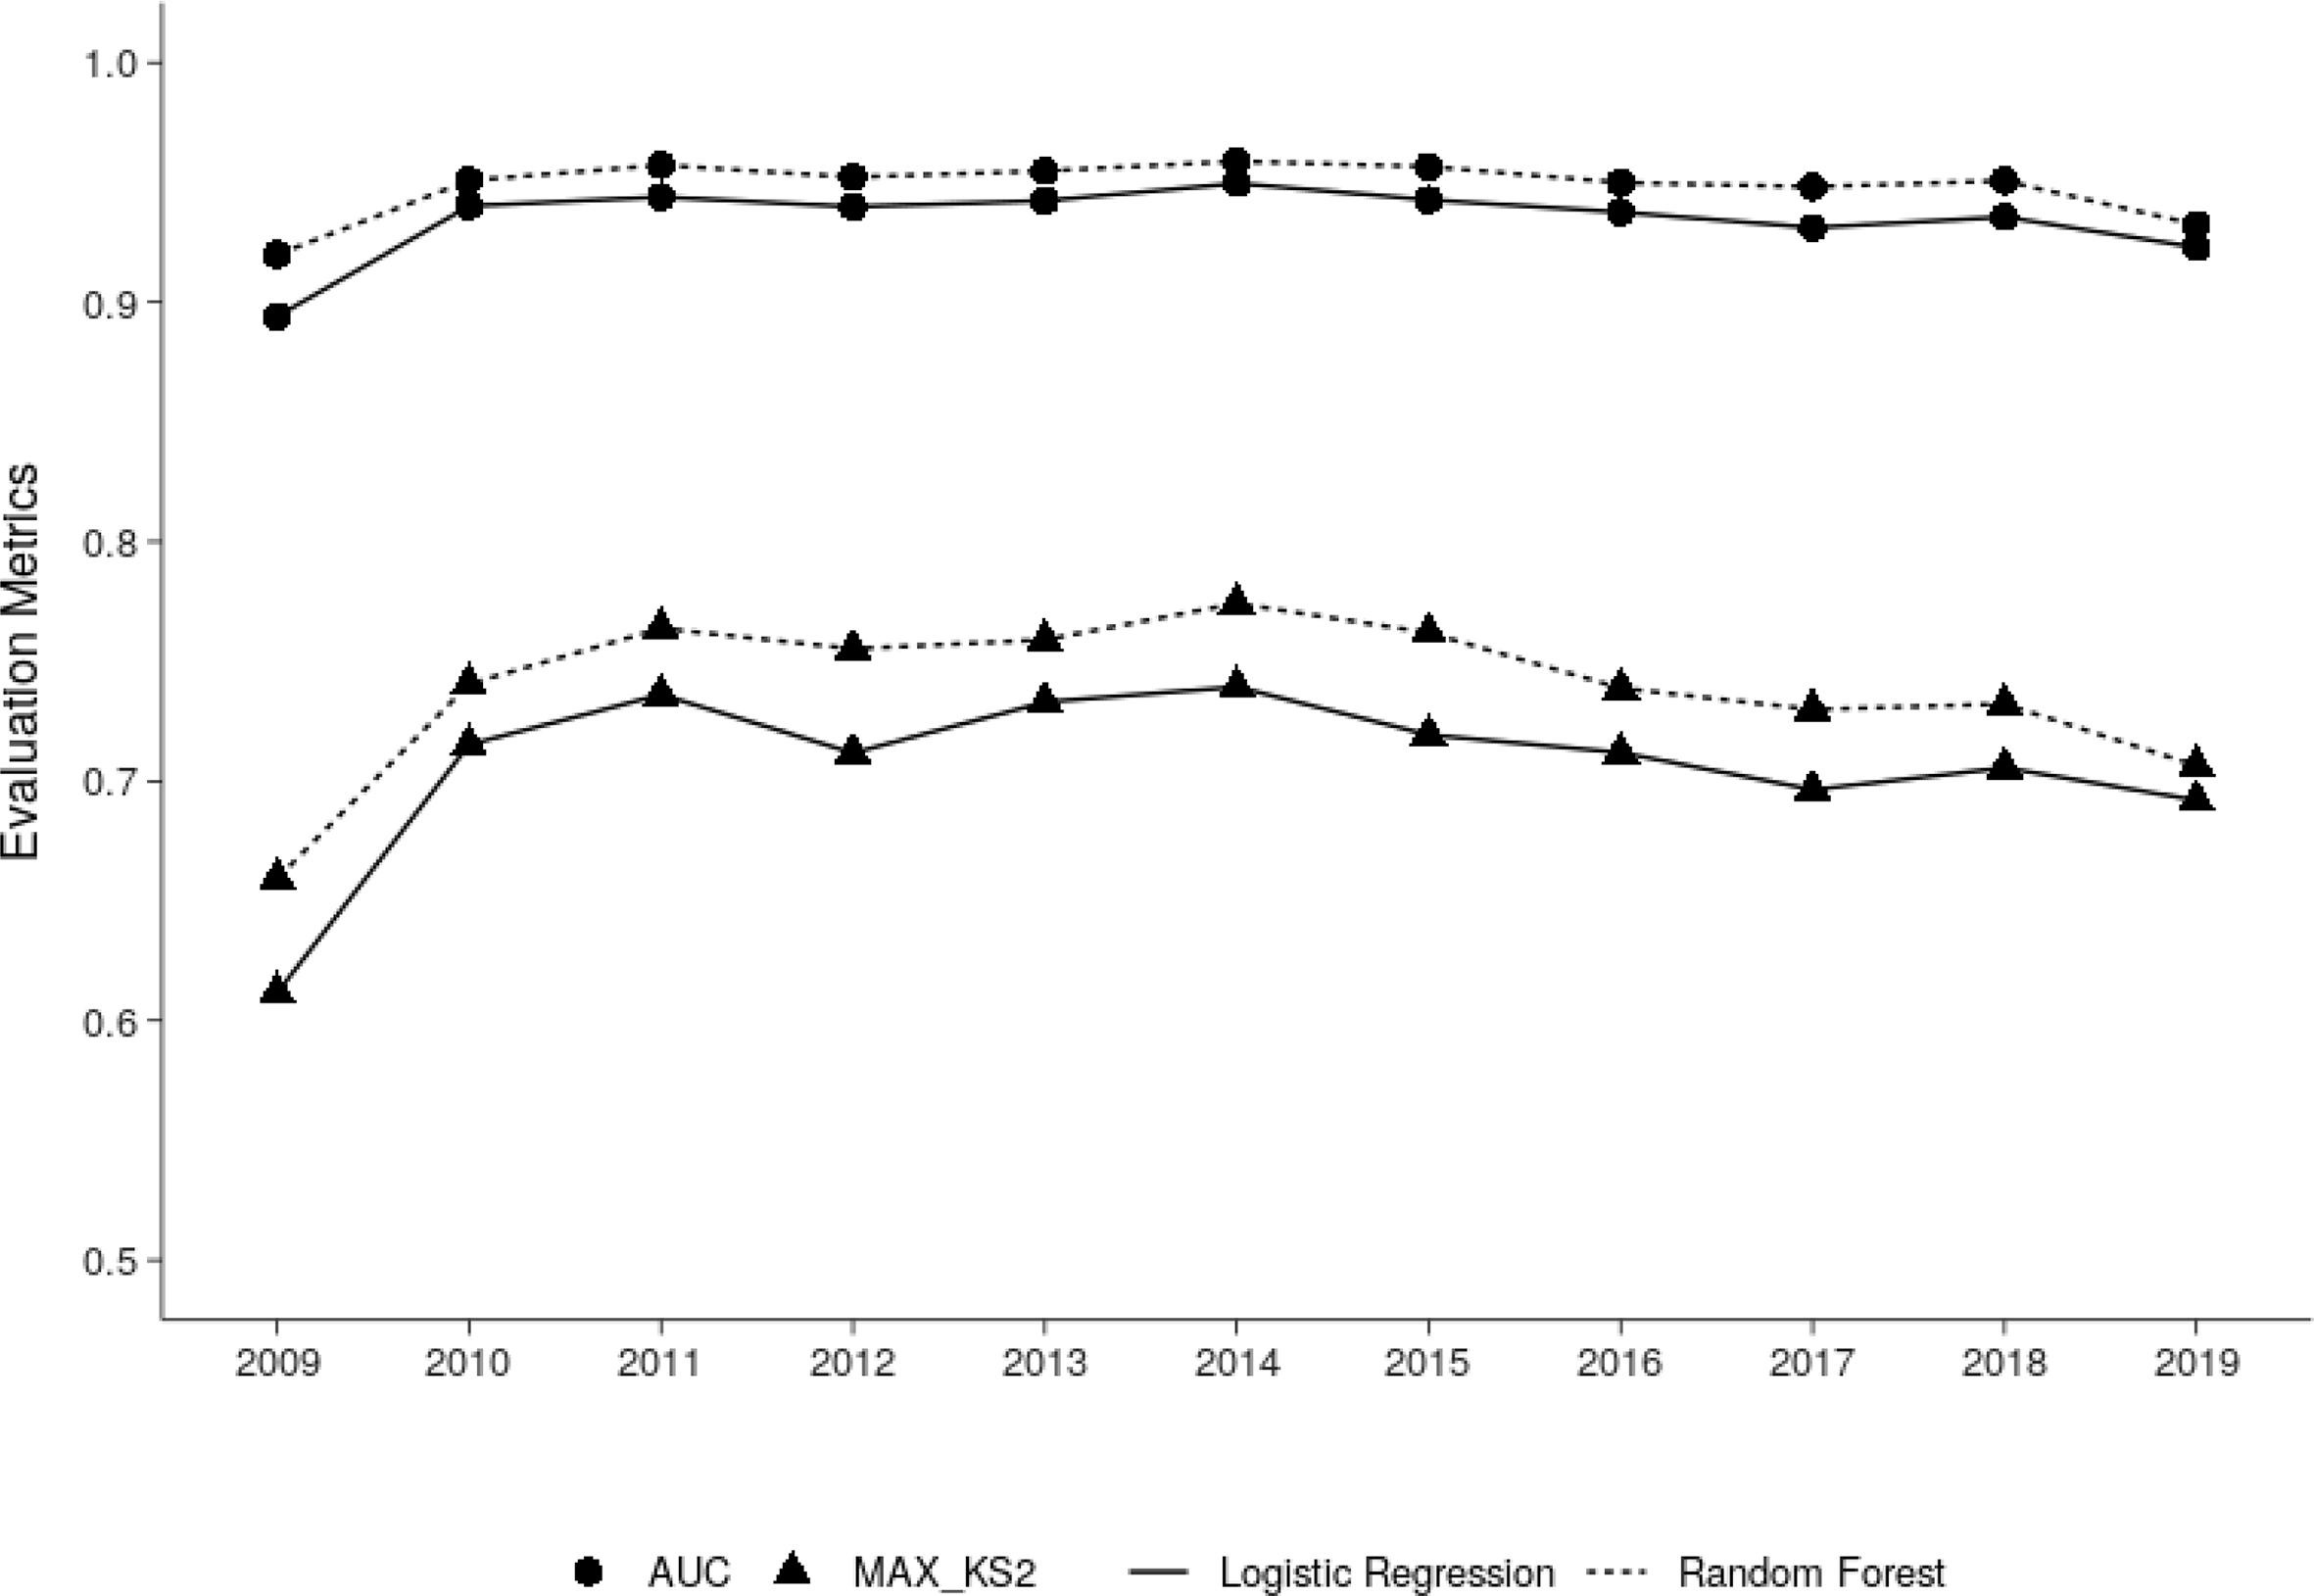
\includegraphics[width=0.9\textwidth]{images/realApplication/performance_models.jpg}}
\par\medskip\ABNTEXfontereduzida\selectfont\textbf{source: self-provided}  
\par\medskip
\end{figure}



Figure \ref{fig:MUA_both_models} presents the feature contribution of both models by the maximum uncentered ALE (MUA). This metric indicates the maximum and isolated influence given the trained data of an underlying feature in predicting school achievement. Both models similarly highlight the well-known determinants of school performance during the whole period, such as \textit{income (per capita)}, \textit{race}, \textit{mother’s education}, \textit{father’s education}, and \textit{students’age} regarding size and direction. This ratifies the most substantial influence of these features on school performance, as has been well-established in the education literature \cite{doi:10.1080/00220671.1997.10544583,   coleman1968equality, coleman2019equality}. It also confirms previous Brazilian studies \cite{Carnoy2022TrendsBrazil} that have used a somewhat different methodology. The \textit{per capita} income significantly influences the likelihood of a school being categorized in the third quartile, with an approximate factor of 0.6. This is roughly three times greater than the impact of parents' education, which holds an estimated factor close to 0.2, over the entire period under study. \textit{Race} has also been significantly related to achievement. While brown students are linked to the school in the lower quartile, white students are linked to higher achievement. Moreover, the feature that indicates the number of computers available to students (\textit{Student's computer}) seems to be a favorable policy with an upward trend (darker points are far from line zero) in classifying schools in the higher quartile, especially in the LR models.

\subsection{Faculty features}

By using the combined analysis, it becomes insightful to explore why certain variables were highlighted in one model but not in another. A LR model, when devoid of explicit interactions, essentially operates as an additive model, capable of emphasizing only the main linear effects of a feature. This appears to be the case for \textit{Faculty education} in Figure \ref{eq:MUA}. Contrary to existing educational studies \cite{doi:10.1080/00220671.1997.10544583, Darling-Hammond2000HowMatters}, \textit{Faculty education} lacks significant explanatory power in LR \ref{eq:MUA}(a) models. The \textit{Faculty education} index, which includes the proportion of teachers with specialization, Master's, and Ph.D. degrees, has increased (from 0.13 in 2009 to 0.18 in 2019) but may not exert uniform impact across all schools. This variation could stem from the differential impact of the index in conjunction with other model features that the RF model could slightly capture. This variation might result from inherent relationships or the diverse efforts of various states in enhancing teacher education levels across the country \cite{SilvaFilho2023LeveragingEducation}. Although there is no feature explicitly representing states, the non-linear effect captured by the RF could be indicated through the proxy behavior of other features.


\begin{figure}[ht!]
\centering
\caption{\textmd{Feature effects size measured by the MUA= from LR (a) and RF (b) in classifying Brazilian secondary
schools using the ENEM score as a performance metric from 2009 to 2019}}
\label{fig:MUA_both_models}
\fcolorbox{gray}{white}{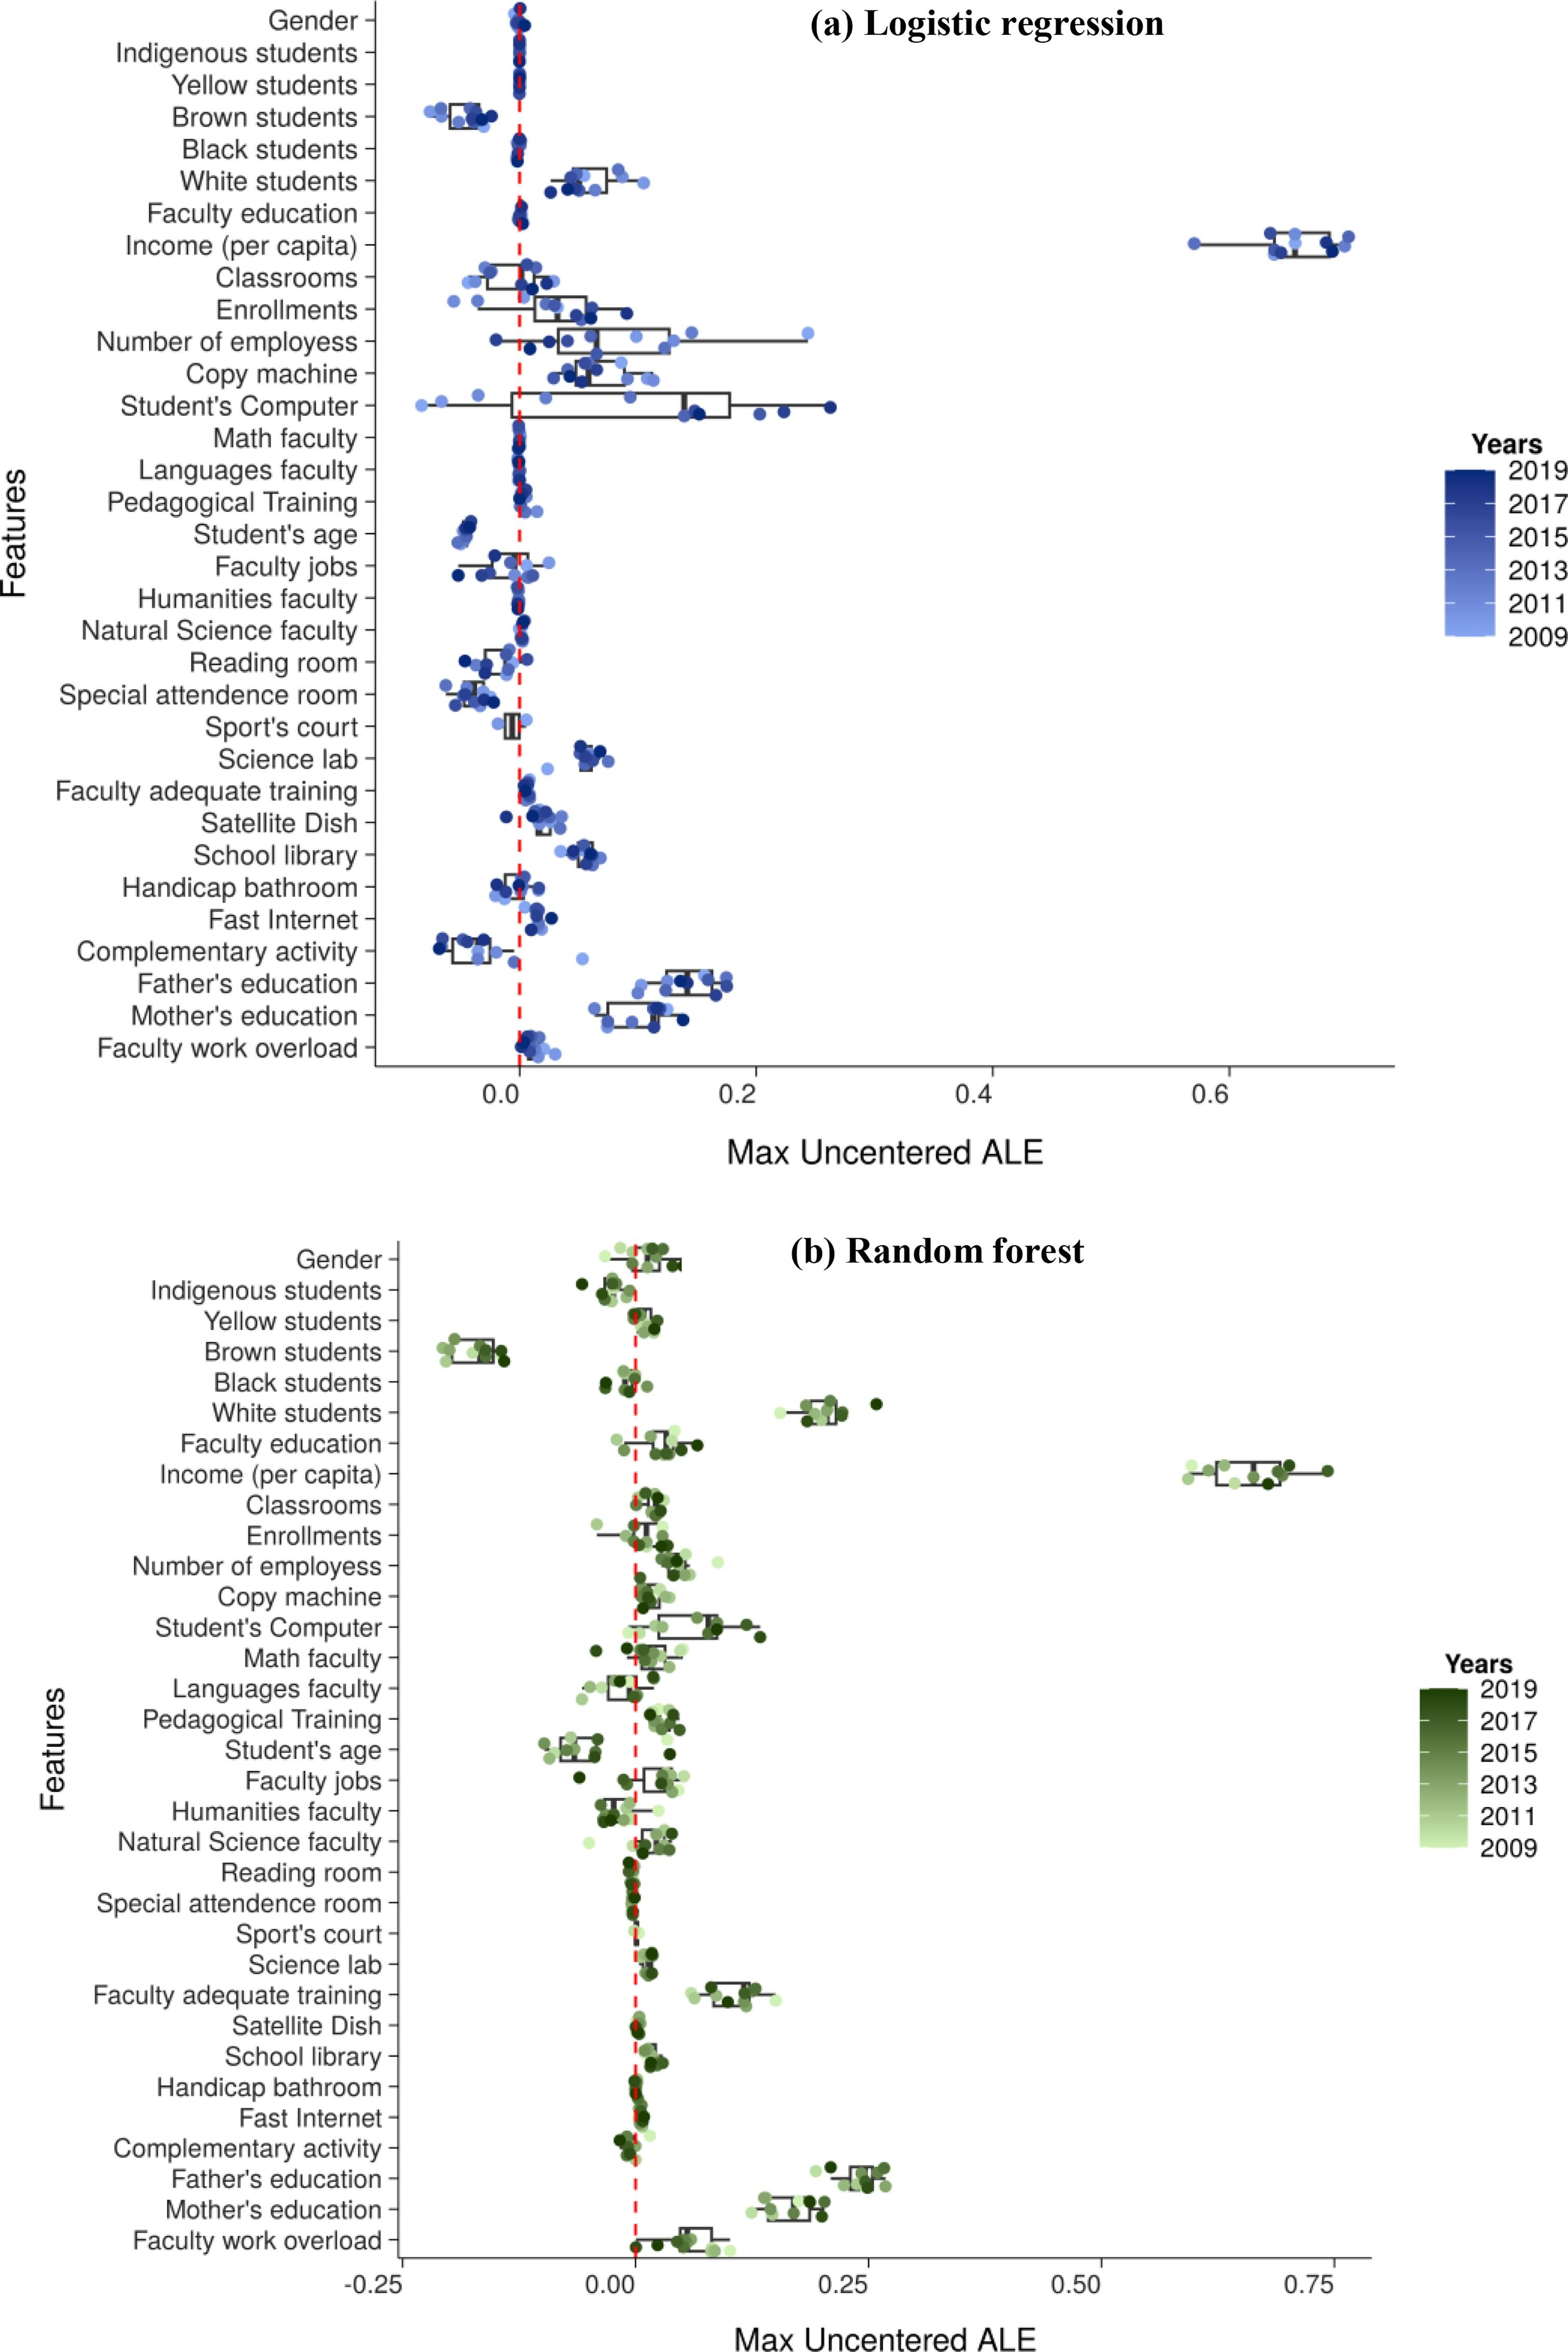
\includegraphics[width=0.9\textwidth]{images/realApplication/variable_relevance_rf_lr.jpg}}
\par\medskip\ABNTEXfontereduzida\selectfont\textbf{Source: self-provided}  
\par\medskip
\end{figure}


Yet in the faculty context, the similar positive size of \textit{Faculty work overload} (equal to 1 when all teachers teach just one subject) and \textit{Faculty adequate training} (equal to 1 when all teachers have an appropriate background in the subjects they teach) in both models suggest that teaching more than one subject is not a problem if they have the appropriate training. On the other hand, the importance of the number of schools where teachers work (\textit{Faculty jobs}) decreases in both models, passing from positive to negative effects. This behavior conforms to earlier qualitative results \cite{Barbosa_2013, Souza2020ODECENAL}.

\subsection{Closer examination of the faculty features}

One relevant way to better understand the specific scenarios is to separate some of the features to observe them more deeply. For example, in Figure \ref{fig:MUA_both_models}, the RF model highlighted some variance among the different faculty areas. These effects seem to derive from a nonlinear relationship with data since the LR model could not find them. Therefore, an additional line plot (Figure \ref{fig:set_variables}) may help to figure out how these features relate. In addition, \textit{Faculty appropriate training} and \textit{Faculty work overload} might enhance the analysis even more. 
As expected, behavior among features related to faculty domains is uneven since they are frequency encoded. Thus, a linear regression was embedded into the plot to obtain a better perception of their trends. The importance of \textit{Natural Science faculty} and \textit{Languages faculty} has increased over time, while the \textit{Math faculty} has taken the opposite direction together with the \textit{Humanities Faculty}. The indexes \textit{Faculty appropriate training} and \textit{Faculty work overload} demonstrate positive importance over the whole period, however with different behaviors. The former is stable with greater importance and seems to be strongly correlated with the \textit{Languages faculty} and \textit{Natural science faculty}. The importance of the latter has been decreasing, as in the case of the \textit{Math faculty} and \textit{Humanities faculty}.
\begin{figure}[ht!]
\centering
\caption{\textmd{ Specific feature effects size measured by MUA related to the faculty.}}
\label{fig:set_variables}
\fcolorbox{gray}{white}{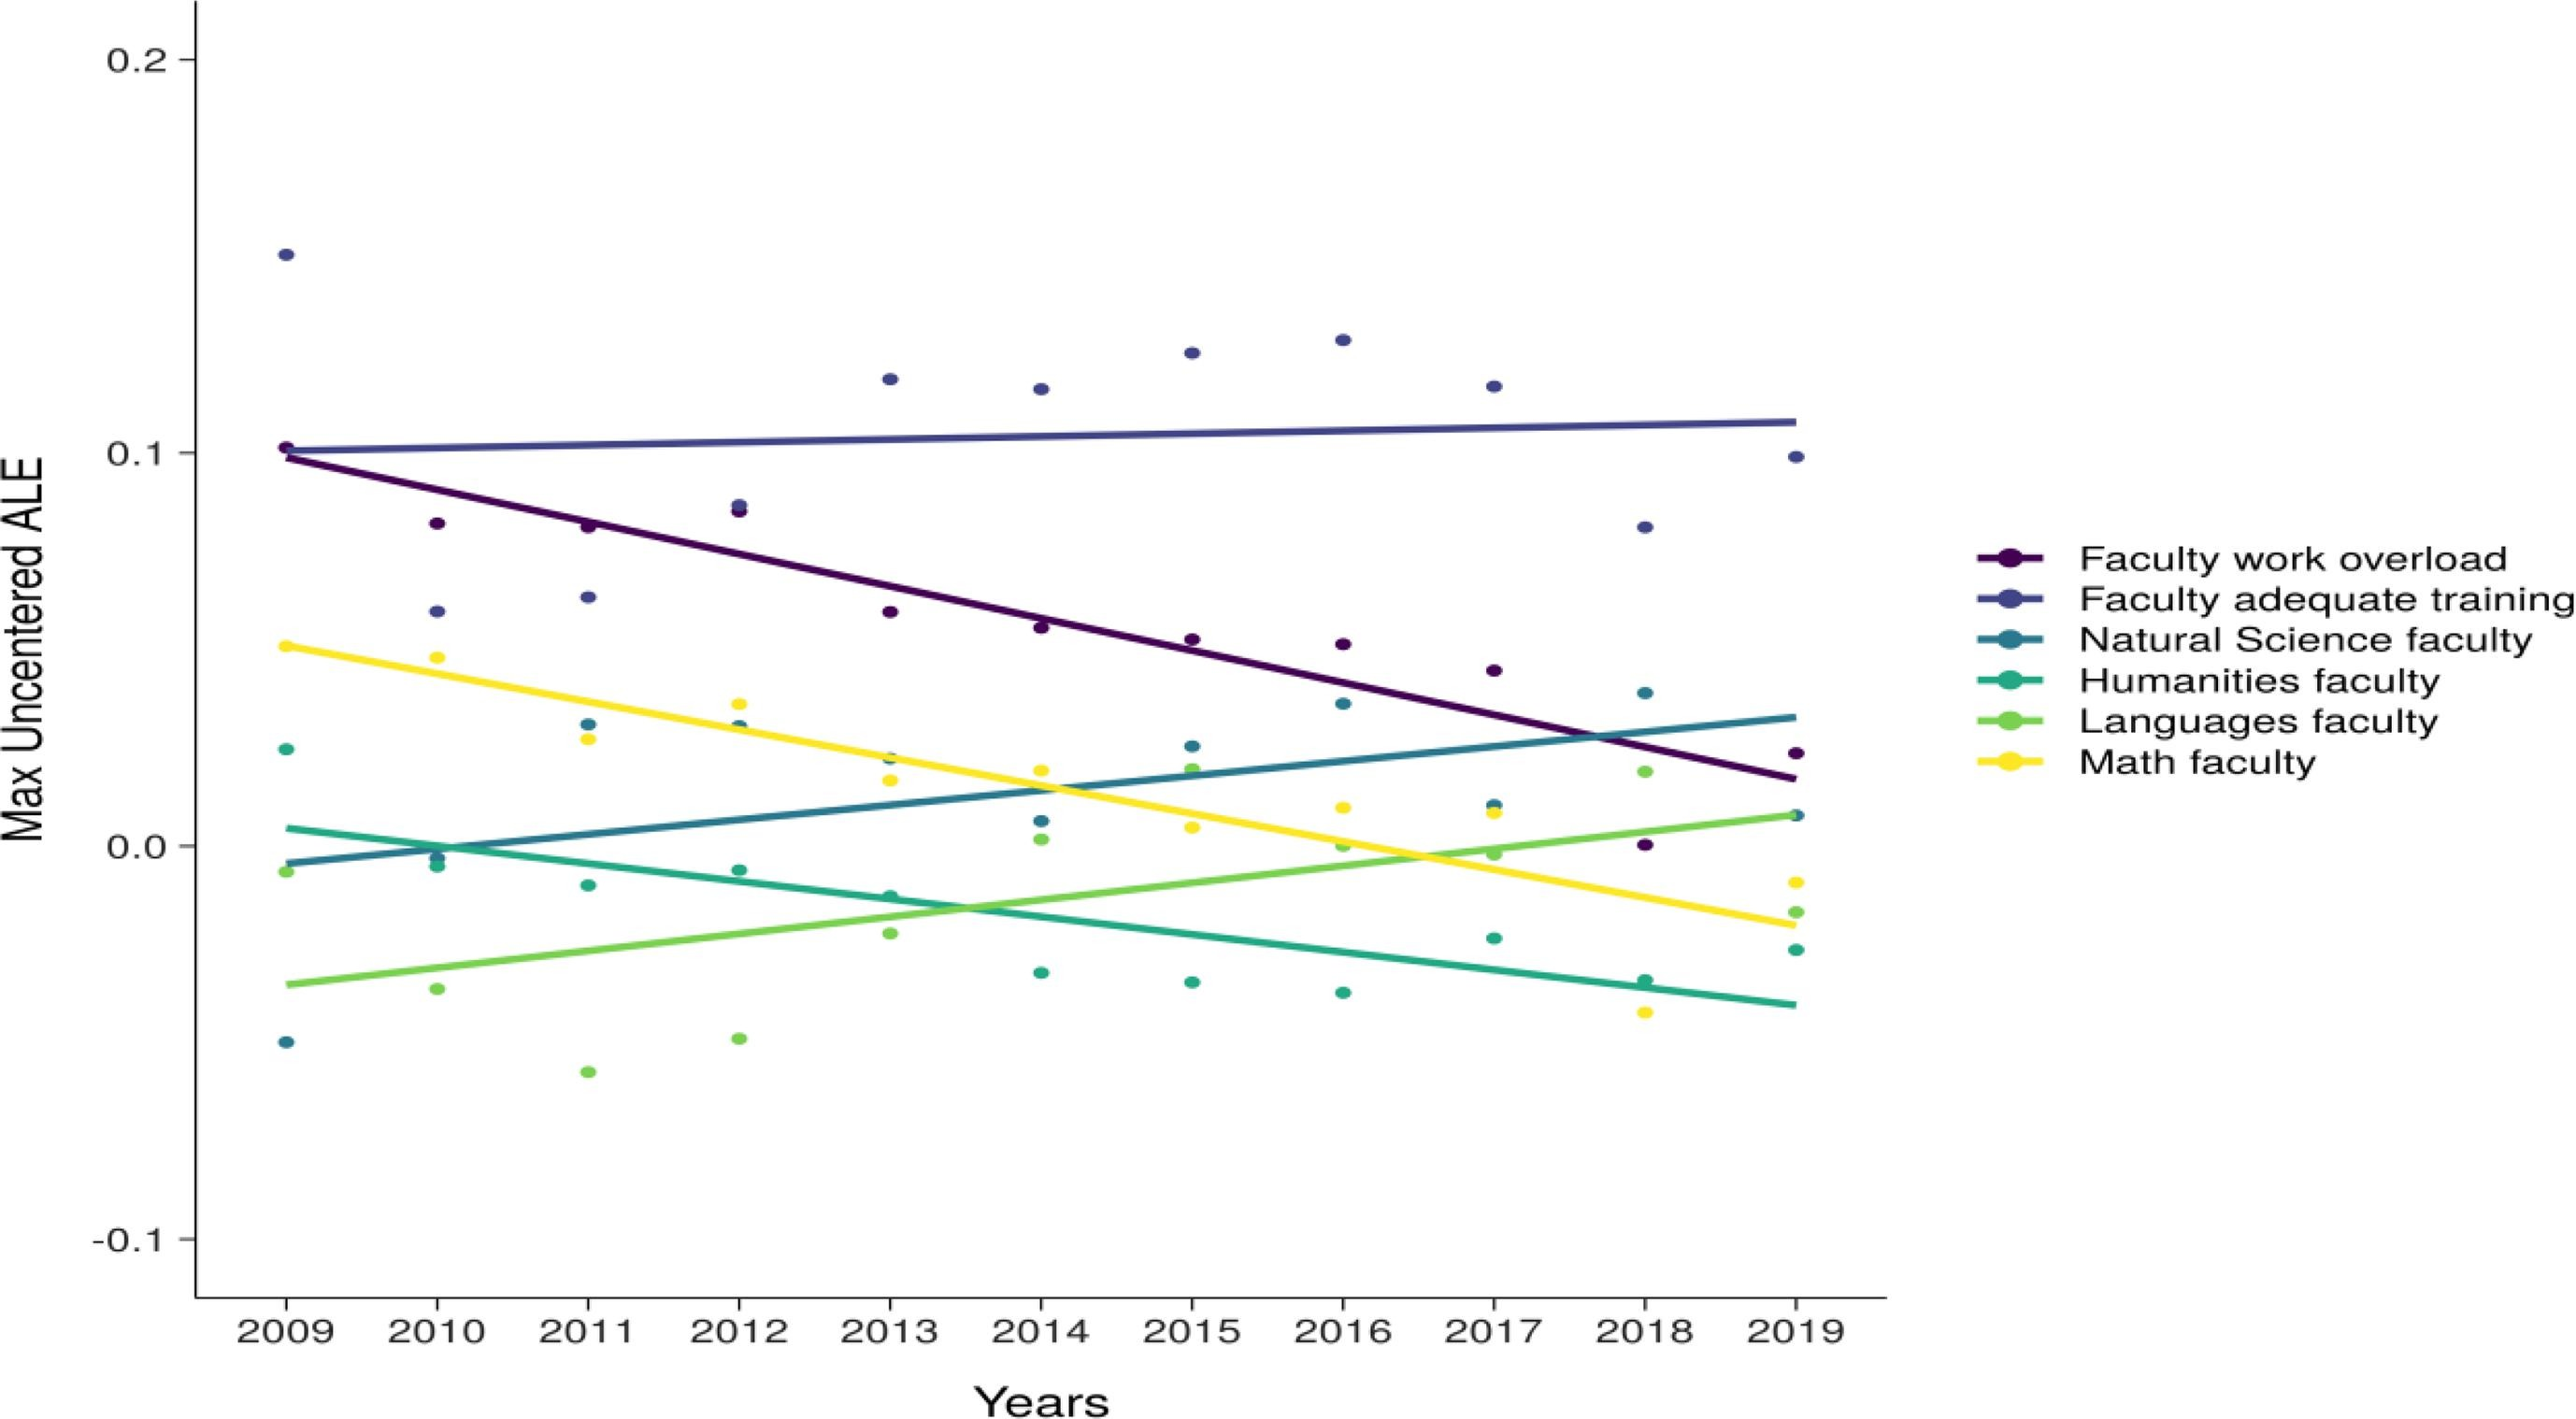
\includegraphics[width=0.9\textwidth]{images/realApplication/set_of_variables.jpg}}
\par\medskip\ABNTEXfontereduzida\selectfont\textbf{source: self-provided}  
\par\medskip
\end{figure}


Figure \ref{fig:matrix_correlation} reveals the behavior detailing the Pearson’s coefficients among the importance of these features. These findings suggest that the importance of the \textit{Math faculty} and \textit{Humanities Faculty} (History, Geography, Philosophy, and Sociology) could be decreasing in some schools due to a heavy workload. Although this is difficult to verify in the training data since it is derived from an unknown nonlinear relationship, the data illustrates that 30\% of humanities teachers teach more than one discipline. Moreover, 90\% of the schools in the final dataset do not report a physics teacher during the period. Thus, it is probable that a math teacher might have to cover this subject, as already reported in  \cite{Santos2012APhysics}. On the other hand, Foreign Languages, Arts, and Physical Education (subjects from the \textit{language domain}) have the lowest indexes for the Faculty adequate training (0.5, 0.6, and 0.7 respectively, against an average of 0.8 for the others), and any endeavor to boost it could be contributing to the slight increase in the importance of \textit{Faculty adequate training} over time. However, these results require caution and more studies with domain expert validation. 

\begin{figure}[ht!]
\centering
\caption{\textmd{Matrix correlation of MUA to the specific set of features related to the faculty.}}
\label{fig:matrix_correlation}
\fcolorbox{gray}{white}{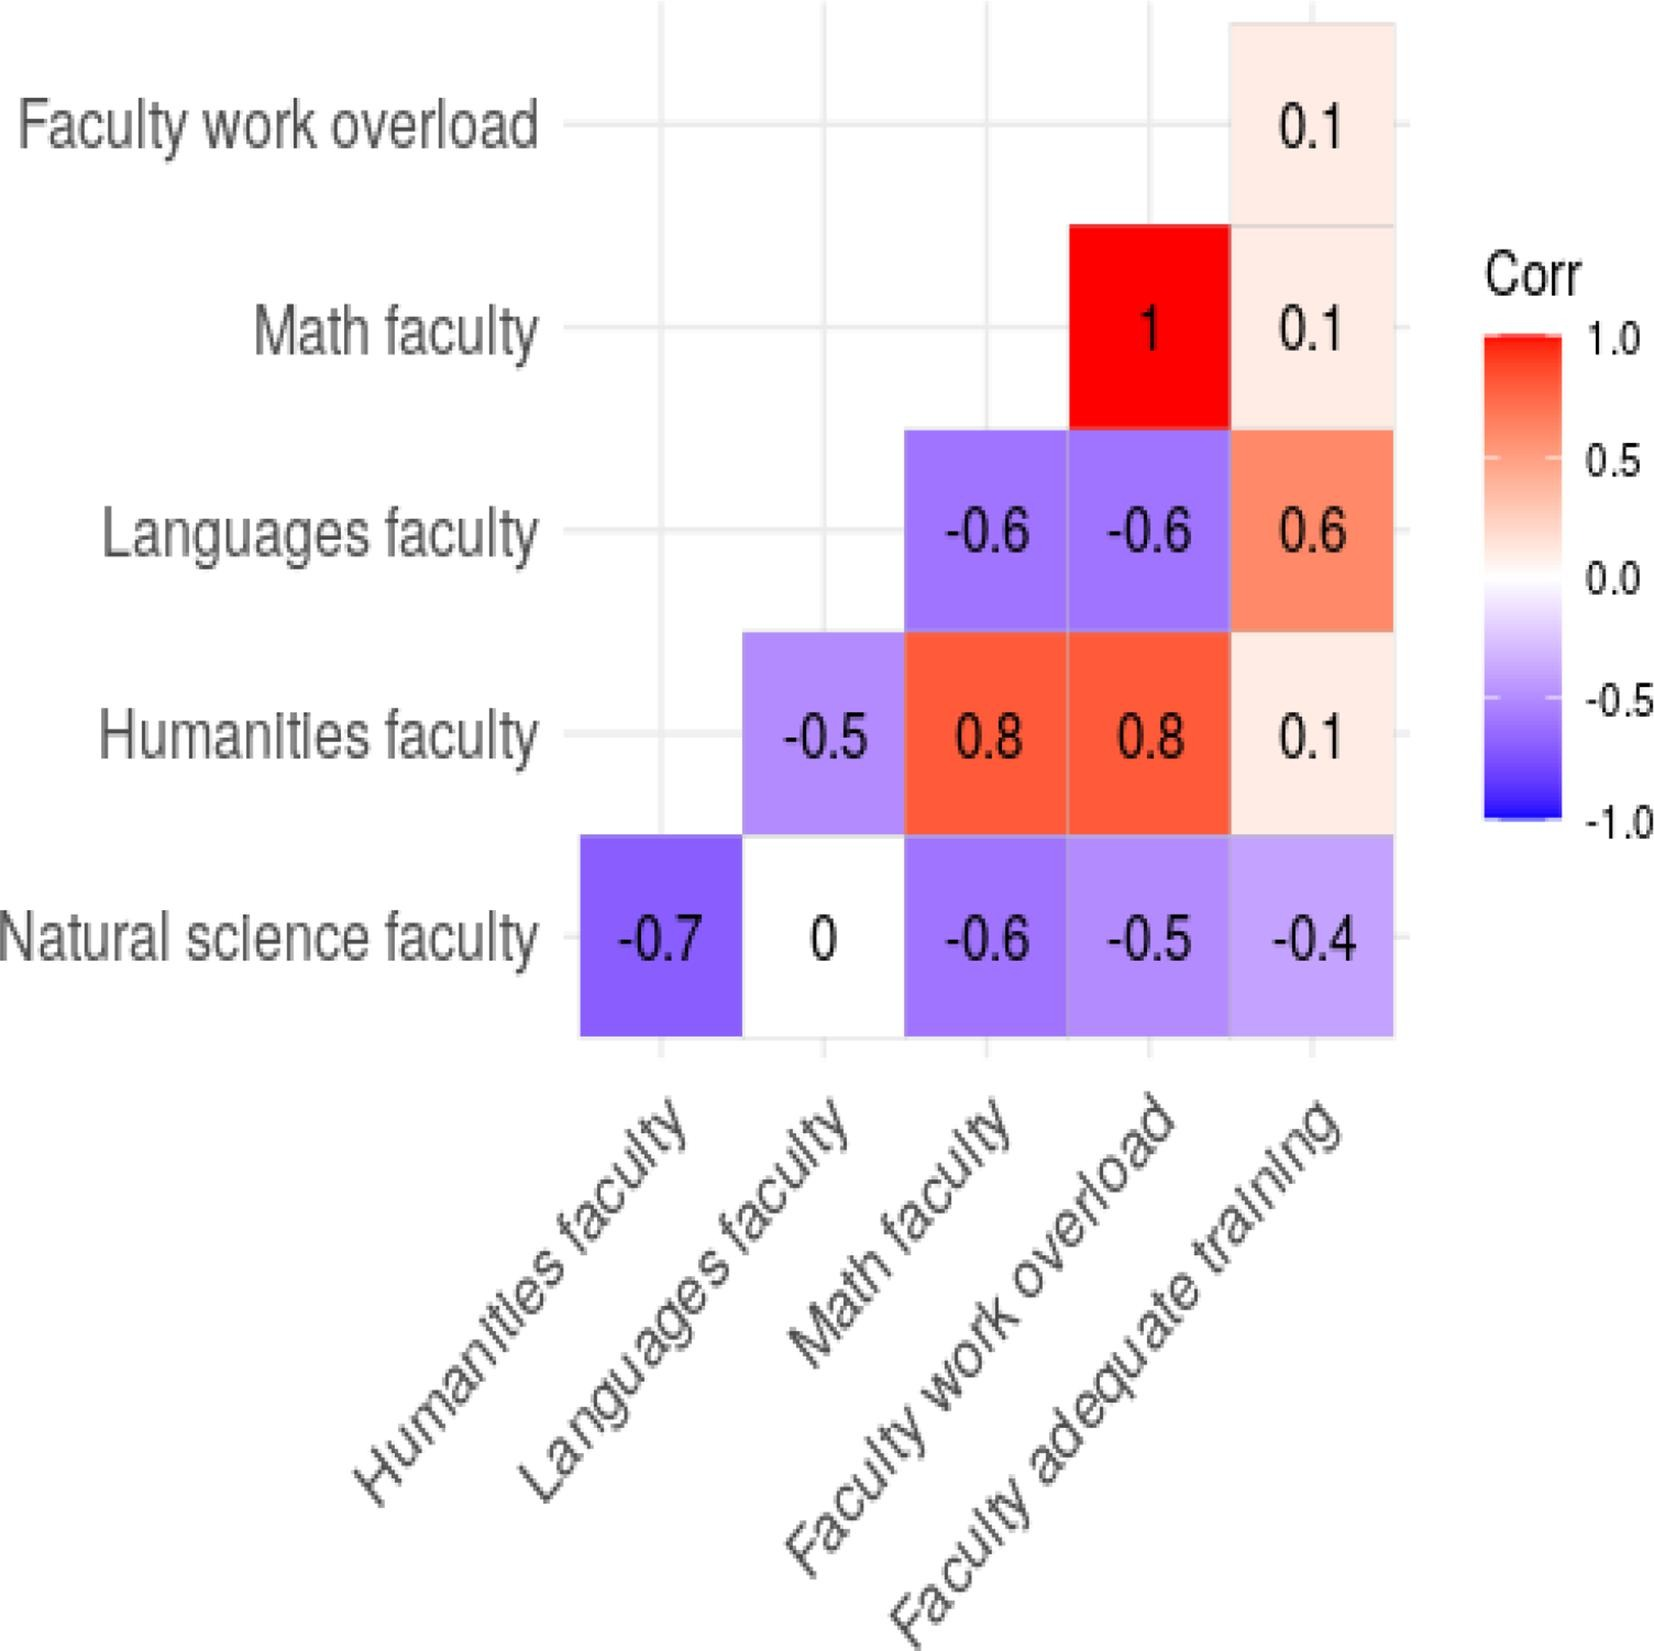
\includegraphics[width=0.7\textwidth]{images/realApplication/matrix_correlation.jpg}}
\par\medskip\ABNTEXfontereduzida\selectfont
\textbf{source: self-provided}  
\par\medskip
\end{figure}

From another perspective, Figure \ref{fig:groups_variable} explains how different combinations of features have influenced school performance during the entire period. It demonstrates the influence of non-actionable features (\textit{race} and \textit{gender}), school features (related to infrastructure), faculty features, and student features (\textit{parents’ education} and \textit{income}) in the period by using a box plot. The metric used is the UAS (on average) from RF models. 

The group of student features has more potential to improve educational performance, followed by the non-actionable features, which have a higher potential for damage. In general, the school features have a low influence, while the teacher features have a limited, although relevant, importance in improving the quality of schools. 

\begin{figure}[ht!]
\centering
\caption{\textmd{Feature effects size measured by UAS (on average) by group regardless of the time.}}
\label{fig:groups_variable}
\fcolorbox{gray}{white}{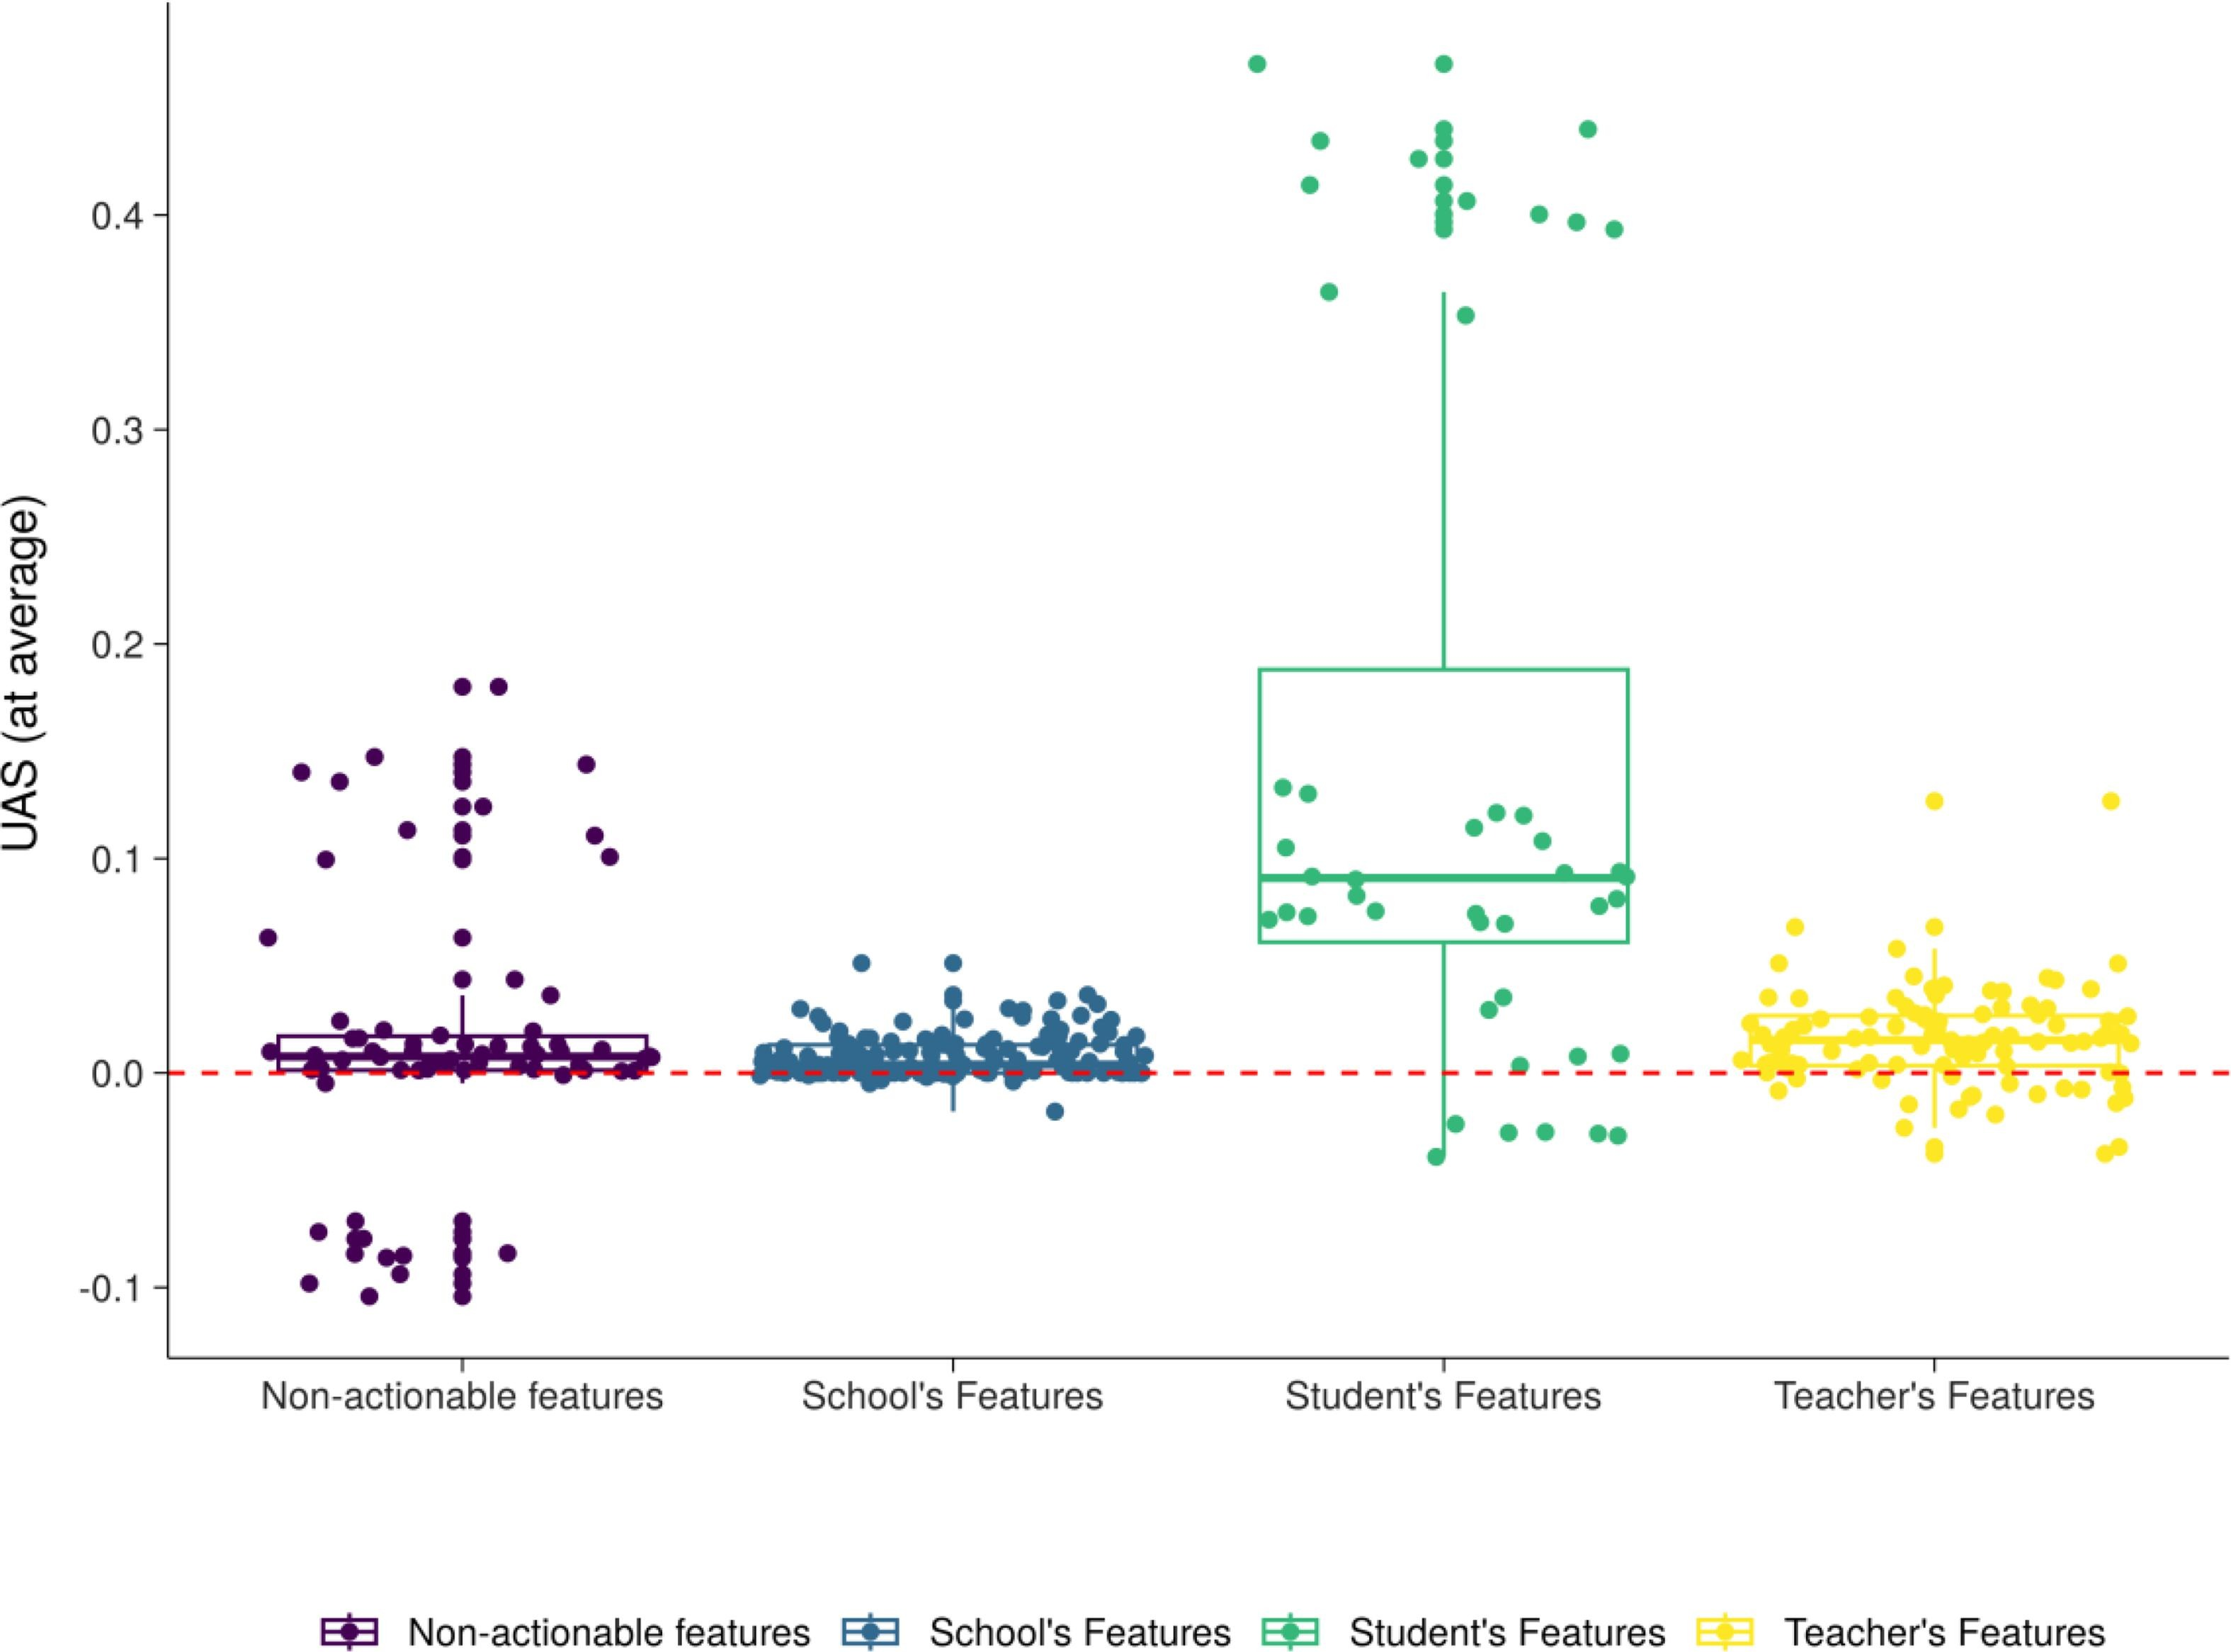
\includegraphics[width=0.9\textwidth]{images/realApplication/groups_variable.jpg}}
\par\medskip\ABNTEXfontereduzida\selectfont\textbf{Source: self-provided}  
\par\medskip
\end{figure}
